
\documentclass[aspectratio=169, 12pt]{beamer}

% -- Theme --------------------------------------------------------------------
\usetheme{Madrid}
\usecolortheme{seahorse}
\setbeamertemplate{navigation symbols}{}
\setbeamertemplate{footline}[frame number]

% -- Packages -----------------------------------------------------------------
\usepackage{amsmath, amssymb}
\usepackage{graphicx}
\usepackage{booktabs}
\usepackage{xcolor}
\usepackage{tikz}
\usepackage{listings}

\graphicspath{{../../plots/}}

% -- Custom colors -------------------------------------------------------------
\definecolor{trivial}{HTML}{d62728}
\definecolor{critical}{HTML}{2ca02c}
\definecolor{topological}{HTML}{1f77b4}
\definecolor{edgemode}{HTML}{e377c2}
\definecolor{codebg}{HTML}{f5f5f5}
\definecolor{codekw}{HTML}{0000cd}
\definecolor{codecomment}{HTML}{228b22}
\definecolor{codestring}{HTML}{8b0000}

\lstset{
  language=Python,
  basicstyle=\ttfamily\footnotesize,
  keywordstyle=\color{codekw}\bfseries,
  commentstyle=\color{codecomment}\itshape,
  stringstyle=\color{codestring},
  backgroundcolor=\color{codebg},
  frame=single,
  framerule=0.4pt,
  rulecolor=\color{gray},
  showstringspaces=false,
  breaklines=true,
  tabsize=4,
}

% -- Macros -------------------------------------------------------------------
\newcommand{\cdag}{c^{\dagger}}
\newcommand{\winding}{\nu}
\newcommand{\ket}[1]{|#1\rangle}
\newcommand{\bra}[1]{\langle#1|}
\newcommand{\Ostring}{X_0 Z_1\cdots Z_{L-2} X_{L-1}}

% -- Title --------------------------------------------------------------------
\title[Kitaev Chain -- Block 3]{Majorana Modes in the Machine}
\subtitle{Week 6: From One Measurement to a Phase Diagram}
\author{Dobromir Stoev\\ Edgar Harutyunyan\\ Guilherme Schewtschik\\ Jaskaran Singh\\ Zhengyi Liu\\ Zhenming Shi}
\institute{Advanced Seminar -- AI-Augmented Theoretical Physics}
\date{\today}

\begin{document}

\begin{frame}
  \titlepage
\end{frame}

\begin{frame}{Week 6 Objective}
  \begin{block}{Goal}
    Turn the Week 5 proof-of-principle into a diagnostic: sweep $\mu$ and ask whether a gate-measurable non-local correlator reconstructs the topological phase boundary.
  \end{block}
  \begin{itemize}
    \item Week 5 measured one sweet-spot example at $t=\Delta$, $\mu=0$.
    \item Week 6 varies $\mu$ across trivial, critical, and topological regimes.
    \item The target observable remains parity-preserving and non-local.
  \end{itemize}
\end{frame}

\begin{frame}{The Observable We Keep}
  \begin{equation*}
    O_{\mathrm{edge}} = \Ostring
  \end{equation*}
  \begin{itemize}
    \item Single-edge operators flip fermion parity, so their expectation vanishes in a parity eigenstate.
    \item The two-edge string preserves parity and probes the correlation between boundary Majoranas.
    \item For $L=4$, this is exactly the Week 5 operator:
    \[
      O_{\mathrm{edge}} = X_0 Z_1 Z_2 X_3.
    \]
  \end{itemize}
\end{frame}

\begin{frame}{Measurement Protocol}
  \begin{columns}[T]
    \begin{column}{0.52\textwidth}
      \textbf{Circuit-level measurement}
      \begin{itemize}
        \item Prepare the ground state with the VQE ansatz.
        \item Rotate qubits with $X$ factors into the $Z$ basis using Hadamards.
        \item Measure all qubits and multiply bit parities to estimate $\langle O_{\mathrm{edge}}\rangle$.
      \end{itemize}
    \end{column}
    \begin{column}{0.44\textwidth}
      \begin{block}{Shot estimator}
        Each shot returns an eigenvalue $m_s = \pm 1$.
        \[
          \langle O\rangle \approx \frac{1}{N}\sum_{s=1}^{N} m_s,
          \qquad
          \sigma \approx \sqrt{\frac{1-\langle O\rangle^2}{N}}
        \]
      \end{block}
    \end{column}
  \end{columns}
\end{frame}

\begin{frame}{Numerical Phase Sweep}
  \centering
  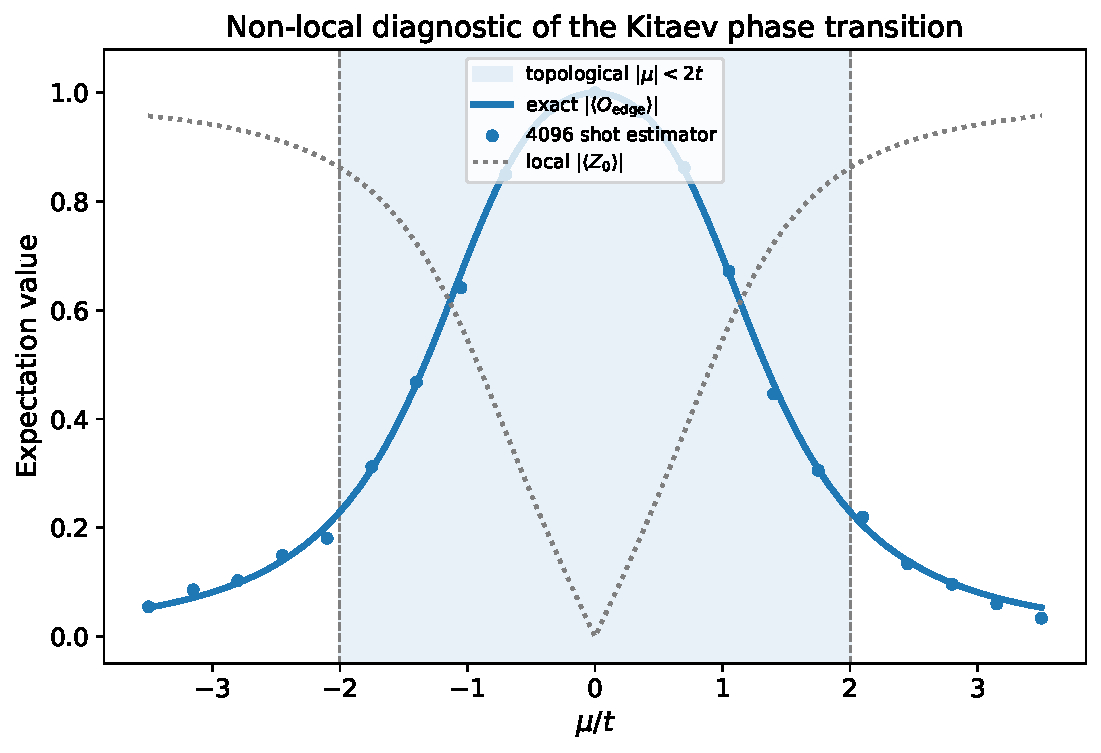
\includegraphics[width=0.95\textwidth]{block3_week6_phase_sweep.pdf}
\end{frame}

\begin{frame}{Reading the Plot}
  \begin{itemize}
    \item The shaded region marks the known topological interval $|\mu| < 2t$.
    \item The non-local edge string is large in the topological regime and drops outside it.
    \item Shot sampling follows the same trend, so the diagnostic is compatible with circuit measurement.
    \item The parity gap gives an independent qubit-Hamiltonian cross-check of the same phase boundary.
  \end{itemize}
\end{frame}

\begin{frame}[fragile]{Implementation Step}
  \begin{lstlisting}[basicstyle=\ttfamily\scriptsize]
for mu in mu_values:
    H = kitaev_qubit_hamiltonian(L, t, mu, delta)
    psi = even_parity_ground_state(H)
    value = <psi| X0 Z1 ... Z(L-2) X(L-1) |psi>
    shot_value = sample_pm_one(value, shots=4096)
  \end{lstlisting}
  \begin{itemize}
    \item Exact diagonalization is still only a small-$L$ validation path.
    \item The measured quantity is the same Pauli string a circuit would estimate from bitstrings.
    \item The next code revision should plug this sweep into the VQE runner directly.
  \end{itemize}
\end{frame}

\begin{frame}{Next: Block 4}
  \begin{itemize}
    \item Add a real VQE loop for every $\mu$ point instead of ED-prepared validation states.
    \item Attach depolarizing, readout, and relaxation noise models to the measurement circuits.
    \item Compare ideal, noisy, and mitigated string-order curves.
    \item Ask how much noise the topological diagnostic tolerates before the phase boundary is lost.
  \end{itemize}
\end{frame}

\end{document}
